\documentclass[a4paper, 10pt]{article}
\usepackage[margin=0.5in]{geometry}
\usepackage{graphicx}
\usepackage{listings}
\usepackage{amsmath}
\usepackage{color}
 
\definecolor{dkgreen}{rgb}{0,0.6,0}
\definecolor{gray}{rgb}{0.5,0.5,0.5}
\definecolor{mauve}{rgb}{0.58,0,0.82}
 
\lstset{ %
  language=Matlab,                % the language of the code
  basicstyle=\footnotesize,           % the size of the fonts that are used for the code
  numbers=left,                   % where to put the line-numbers
  numberstyle=\tiny\color{gray},  % the style that is used for the line-numbers
  stepnumber=2,                   % the step between two line-numbers. If it's 1, each line 
                                  % will be numbered
  numbersep=5pt,                  % how far the line-numbers are from the code
  backgroundcolor=\color{white},      % choose the background color. You must add \usepackage{color}
  showspaces=false,               % show spaces adding particular underscores
  showstringspaces=false,         % underline spaces within strings
  showtabs=false,                 % show tabs within strings adding particular underscores
  frame=single,                   % adds a frame around the code
  rulecolor=\color{black},        % if not set, the frame-color may be changed on line-breaks within not-black text (e.g. commens (green here))
  tabsize=2,                      % sets default tabsize to 2 spaces
  captionpos=b,                   % sets the caption-position to bottom
  breaklines=true,                % sets automatic line breaking
  breakatwhitespace=false,        % sets if automatic breaks should only happen at whitespace
  title=\lstname,                   % show the filename of files included with \lstinputlisting;
                                  % also try caption instead of title
  keywordstyle=\color{blue},          % keyword style
  commentstyle=\color{dkgreen},       % comment style
  stringstyle=\color{mauve},         % string literal style
  escapeinside={\%*}{*)},            % if you want to add a comment within your code
  morekeywords={*,...}               % if you want to add more keywords to the set
}
\begin{document}
\title {Pattern Recognition EN2202 \\ Assignment 2}
\author{Radu-Mihai Pana-Talpeanu rmpt@kth.se \\Maria Gerontini mger@kth.se}
\maketitle

\section{Feature Extraction}
In this part of the project, the goal was to decide on a well-suited feature representation for the sequence of vectors that an HMM will receive as input. Our theme is online single character recognition which means that as raw data we have the x,y coordinate representation of the drawn points and a pen-up bit.

In order to get a feature vector almost similar for any kind of characters will be written we needed a normalisation step. For that reason we normalised all the written characters by their size and by their location. 

After that we had to found the way we will represent the features and what kind of features we need to use. During an extensively research we decided that we should use the directions , the length of each stroke or segment and the relative position between the end of one pen stroke and the start of the next.  A character consists by one or more strokes. By the term strokes we mean the lines from a first penDown until the first penUp. Below is the description for each feature.

\subsection{Directions}
We determined the line direction between two adjacent positions in one stroke of a character and in the case of one stroke character we determined the direction for each segment.  We used this segment technique for our one stroke character because in another way we would have only one type of directions  e.g 'C' has only South and there was high possibility for misclassifications with 'O' or 'I'.  Then we used 8 directions ,for simplifying  reasons, to encode the directions into e.g East (0) North(2), NorthEast(1), etc. and then we encoded these directions respectively to the Fig.1 The direction are determined by the equation below where the Y and X are the normalised coordinates from the previous step.  These features can be found on the first row of our feature vector.


\[
tan \vartheta = (y{}_t - y_{t-1} )/(x{}_t - x_{t-1}) .
\]

\begin{figure}[h!]
  \caption{Directions}
  \centering
    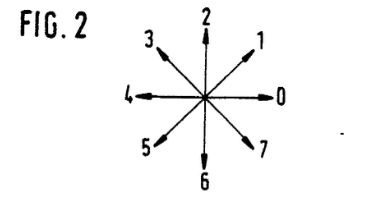
\includegraphics[width=0.5\textwidth]{directions}
\end{figure}

\subsection{Length of stroke}
In order to achieve better prediction results we used the stroke length or the segment length. See the following equation.
\[
Length = \sqrt{a ^2 + b^2} 
\]
\[
a = y{}_t - y_{t-1}
b = x{}_t - x_{t-1}
\] 
We then encoded this Length to 4 different classes based on the normalised size C we used on the normalisation step.
\begin{figure}[h!]
  \caption{Length Code}
  \centering
    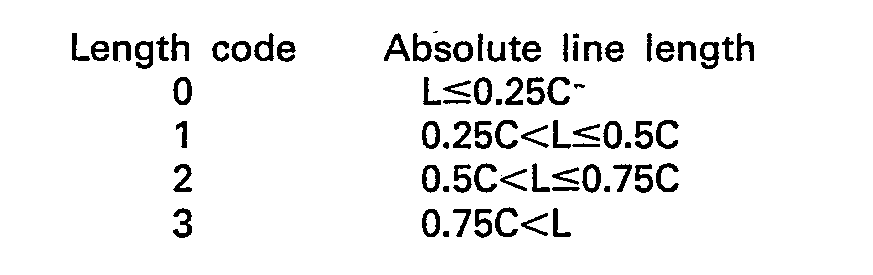
\includegraphics[width=0.5\textwidth]{lengthcode}
\end{figure}

In this way we can have more accurate features for each time step. For example in the case of letter 'A' the feature vector has 3 strokes the two of them have the biggest length category 3 and the middle has the lowest length class 0. So we can be sure that this letter is an A and we can distinguish it from the letter K which has also 3 strokes but with 2 shorter lines and one bigger than the other. In addition to this, that type of feature gives us the opportunity to distinguish characters like 'T' and '+' as long as T contains two strokes the one shorter than the other while the '+' has two strokes almost with the same length. This type of feature can be found at the second row of our feature vector.


\subsection{Relative Position of penUp and penDown}
Finally, we used the relative position of the penDown feature from the previous penUp. This feature is very essential in order to be able to distinguish characters like 'T' and '+' where their only difference is the offset between the two vertical and the horizontal lines. As a result with this feature combined with the Length code we are able to separate these two characters. These coordinates can be found at the 3rd and the 4th row of our feature vector when a penDown occurs after a penUp session.

At the end , we need to mention that we don't take into account any features during a penUp session for that reason we set there values with no meaning like the value -1.

So a typical example of our feature Vector is below.
\begin{table}
    \begin{tabular}{|l|l|l|l|l|}
        \hline
        Directions  & 5 & 5 & -1 & 0     \\ \hline
        Length Code & 0 & 0 & -1 & 3     \\ 
        X PenDown   & 0 & 0 & 0  & 0.345 \\ 
        Y PenDown   & 0 & 0 & 0  & 0.456 \\
        \hline
    \end{tabular}
\end{table}




\end{document}
